%%%%%%%%%%%%%%%%%%%%%%%%%%%%%%%%%%%%%%%%%
% Short Sectioned Assignment
% LaTeX Template
% Version 1.0 (5/5/12)
%
% This template has been downloaded from:
% http://www.LaTeXTemplates.com
%
% Original author:
% Frits Wenneker (http://www.howtotex.com)
%
% License:
% CC BY-NC-SA 3.0 (http://creativecommons.org/licenses/by-nc-sa/3.0/)
%
%%%%%%%%%%%%%%%%%%%%%%%%%%%%%%%%%%%%%%%%%

%----------------------------------------------------------------------------------------
%	PACKAGES AND OTHER DOCUMENT CONFIGURATIONS
%----------------------------------------------------------------------------------------

\documentclass[paper=a4, fontsize=11pt]{scrartcl} % A4 paper and 11pt font size

\usepackage[T1]{fontenc} % Use 8-bit encoding that has 256 glyphs
\usepackage{fourier} % Use the Adobe Utopia font for the document - comment this line to return to the LaTeX default
\usepackage[english]{babel} % English language/hyphenation
\usepackage{amsmath,amsfonts,amsthm} % Math packages
\usepackage{slashed}

\usepackage{graphicx}
\usepackage{multicol}
\usepackage{enumitem}
\usepackage{caption}
\usepackage{esint}

\usepackage{listings}
\usepackage{color}

\definecolor{dkgreen}{rgb}{0,0.6,0}
\definecolor{gray}{rgb}{0.5,0.5,0.5}
\definecolor{mauve}{rgb}{0.58,0,0.82}

\lstset{frame=tb,
  language=C,
  aboveskip=3mm,
  belowskip=3mm,
  showstringspaces=false,
  columns=flexible,
  basicstyle={\small\ttfamily},
  numbers=none,
  numberstyle=\tiny\color{gray},
  keywordstyle=\color{blue},
  commentstyle=\color{dkgreen},
  stringstyle=\color{mauve},
  breaklines=true,
  breakatwhitespace=true
  tabsize=3
}

\usepackage{lipsum} % Used for inserting dummy 'Lorem ipsum' text into the template

\usepackage{sectsty} % Allows customizing section commands
\allsectionsfont{\centering \normalfont\scshape} % Make all sections centered, the default font and small caps

\usepackage{abstract}
\renewcommand{\abstractnamefont}{\normalfont\Large}
\renewcommand{\abstracttextfont}{\normalfont}

\usepackage{fancyhdr} % Custom headers and footers
\pagestyle{fancyplain} % Makes all pages in the document conform to the custom headers and footers
\fancyhead{} % No page header - if you want one, create it in the same way as the footers below
\fancyfoot[L]{} % Empty left footer
\fancyfoot[C]{} % Empty center footer
\fancyfoot[R]{\thepage} % Page numbering for right footer
\renewcommand{\headrulewidth}{0pt} % Remove header underlines
\renewcommand{\footrulewidth}{0pt} % Remove footer underlines
\setlength{\headheight}{13.6pt} % Customize the height of the header

\numberwithin{equation}{section} % Number equations within sections (i.e. 1.1, 1.2, 2.1, 2.2 instead of 1, 2, 3, 4)
\numberwithin{figure}{section} % Number figures within sections (i.e. 1.1, 1.2, 2.1, 2.2 instead of 1, 2, 3, 4)
\numberwithin{table}{section} % Number tables within sections (i.e. 1.1, 1.2, 2.1, 2.2 instead of 1, 2, 3, 4)

%\setlength\parindent{0pt}  Removes all indentation from paragraphs - comment this line for an assignment with lots of text

%Average
\newcommand{\average}[1]{\ensuremath{\left\langle #1 \right\rangle}}
%Parenthesis 
\newcommand{\parentheses}[1]{\ensuremath{\left( #1 \right)}}
%Commutator
\newcommand{\commutator}[1]{\ensuremath{\left[ #1 \right]}}
%Anti-commutator
\newcommand{\anticommutator}[1]{\ensuremath{\left\lbrace #1 \right\rbrace}}
%QED
\newcommand{\QED}{\begin{flushright}\textit{Q.E.D.}\end{flushright}}
%Split
\newcommand{\spliteq}[1]{\begin{split} #1 \end{split}}
%----------------------------------------------------------------------------------------
%	TITLE SECTION
%----------------------------------------------------------------------------------------

\newcommand{\horrule}[1]{\rule{\linewidth}{#1}} % Create horizontal rule command with 1 argument of height

\title{
\vspace{-2.5cm}
\begin{center}

\includegraphics[width=2.5cm]{logo-kth.png}\\[-1mm]
\hspace{-3mm}
\end{center}
\normalfont \normalsize
\textsc{Theoretical Physics} \\ [25pt] % Your university, school and/or department name(s)
\horrule{0.5pt} \\[0.4cm] % Thin top horizontal rule
\huge Quantum Field Theory\\ % Course name
SI2410\\ % Course code
\huge Fall 2014\\ % Semester
\huge Preparation Questions \\ % The assignment title
\horrule{2pt} \\[0.5cm] % Thick bottom horizontal rule
}

\author{David Aceituno, David Blomqvist,
\\ Fredrik Hanse, Erik Holmgren, Jens Wir\'{e}n}
\date{\normalsize\today} % Today's date or a custom date

\begin{document}

\maketitle % Print the title

%----------------------------------------------------------------------------------------

\section{Seminar 1: Functional integrals and introduction to renormalization}

\subsection{What is the relationship between the functional integral formalism and
the n-point correlation function?}
General generating functional is given by

\begin{equation}
Z[J]=\int D\phi \exp \left[i\int d^4x[L+J(x)\phi(x)] \right]
\end{equation}

where $L$ is the Lagrangian density and $J(x)\phi(x)$ is a source term.

The n-point correlation function is then given by

\begin{equation}
\left\langle 0 | T \phi (x_1) ... \phi (x_n) | 0 \right\rangle = \dfrac{1}{Z_0} \prod_{i=1}^{n} \parentheses{-i\dfrac{\delta}{\delta J(x_i)} Z[J]}
\end{equation}

where $Z_0=Z[J=0]$. This yields

\begin{equation}
\left\langle 0 | T \phi (x_1) ... \phi (x_n) | 0 \right\rangle = \dfrac{\int D\phi \phi(x_1)...\phi(x_n) \exp \left[i\int d^4xL \right]}{\int D\phi \exp \left[i\int d^4xL \right]}
\end{equation}

\subsection{Given a Lagrangian density, how can the Feynman rules of a theory be
computed using functional integral formalism?}
The Feynman rules can be computed by Taylor expanding

\begin{equation}
\exp [iS] = \exp \commutator{i \int d^4 x L_0 + L_{int}}
\end{equation}

where $S$ is the action, $L_0$ is the free Lagrangian density and $L_{int}$ is the interaction Lagrangian density. In the case of $\lambda \phi^4$-theory we have the Lagrangian

\begin{equation}
L=L_0-\dfrac{\lambda}{4!}\phi^4
\end{equation}

and by Taylor expansion

\begin{equation}
\exp iS = \exp \commutator{i \int d^4 x \parentheses{L_0 - \dfrac{\lambda}{4!}\phi^4}}= \exp \commutator{i \int d^4 x L_0} \parentheses{1-i\int d^4x \dfrac{\lambda}{4!}\phi^4+...}
\end{equation}

where $L_0$ gives the propagators and all terms of order higher than two yields interaction. In this case we read of the vertex factor in momentum space as

\begin{equation}
-i\lambda (2 \pi)^4 \delta ^{4} \parentheses{\sum p}
\end{equation}

\subsection{What complications arise when using the functional integral formalism to
quantize the electromagnetic field? How is it solved?}
In QED the functional integral,
\begin{equation}
\int DA e^{iS[A]}
\end{equation}
is badly defined because we are redundantly integrating over a continuous infinity of physically equivalent field configurations. This happens when S[A] = 0 due to gauge invariance, 
\begin{equation}
A_{\mu} \rightarrow A_{\mu} + \frac{1}{e} \partial_{\mu} \alpha (x)
\end{equation}
and thus $ A_{\mu} = \frac{1}{e} \partial_{\mu} \alpha (x)$ is equal to $A_{\mu} = 0$. Through the Faddeev-Popov procedure we introduce some gauge fixing function G(A) = 0, this would be G(A) = $\partial_{\mu} A^{\mu}$ in the Lorentz gauge. We can insert a functional delta function $\delta (G(A))$ into our functional integral by using,
\begin{equation}
1 = \int D\alpha ~ \delta(G(A^{\alpha}))det\left[ \frac{\delta G}{\delta \alpha}\right]
\end{equation}
and a general G given by, $G(A) = \partial^{\mu} A_{\mu} - \omega (x)$ where $\omega$ is some scalar function. This gives the photon propagator as,
\begin{equation}
\tilde{D}^{\mu \nu}_F (k) = \frac{-i}{k^2+i\epsilon} \left( g^{ \mu \nu} - (1-\xi) \frac{k^{\mu}k^{\nu}}{k^2}\right)
\end{equation}
where the choice of $\xi$ gives our gauge.

\subsection{What are the properties of Grassmann numbers and how are they used to
quantize spinor fields?}
The Grassman numbers are anticommuting numbers with the following properties,

\begin{equation}
\begin{split}
\theta \eta = - \eta \theta \\
\theta^2 = 0 \\
\int 1 d\theta = 0 \\
\int \theta d\theta = 1 \\
\int \frac{\partial f}{\partial \theta} d\theta = 0
\end{split}
\end{equation}

To quantize spinor fields a grassman valued source field is introduced into $Z[\eta, \bar{\eta}]$ such that, 
\begin{equation}
Z[\eta, \bar{\eta}] = \int D \psi \int D \bar{\psi} e^{i\int d^4 x [L + \bar{\eta}\psi+ \bar{\psi}\eta ]}.
\end{equation}
A Grassman field is given by,
\begin{equation}
\eta (x) = \sum_i \eta_i \phi_i
\end{equation}
where $\eta_i$ is a grassman number and $\phi_i$ is a field basis and in the equation above the base is 4-spinor Dirac fields. 

\subsection{What is the superficial degree of divergence and how can it be computed?
Use QED as an example.}
The superficial degree of divergence is for a Feynmann diagram's integral defined as,
\begin{equation}
D = (\text{power of momenta in numerator} - \text{power of momenta in denominator})
\end{equation}
and tells us something about the divergence of a given diagram. In general d-dimensional QED this can be written as,
\begin{equation}
D = d + \frac{d-4}{2}V - \frac{d-2}{2}N_{\gamma} - \frac{d-1}{2}N_{e}
\end{equation} 
where V is the number of vertices and $N_i$ the number of i = photon, electron external lines. D does not tell us everything about the divergence, in QED the three diagrams (c,f and g in Fig. \ref{fig:divergent_diagrams_QED}) always diverge, D can only tell us if a given diagram diverge or not if the diagram does not contain any of those three. However for any theory we can always remove the divergent subdiagrams and D holds.

\begin{figure}[hbtp]
\centering
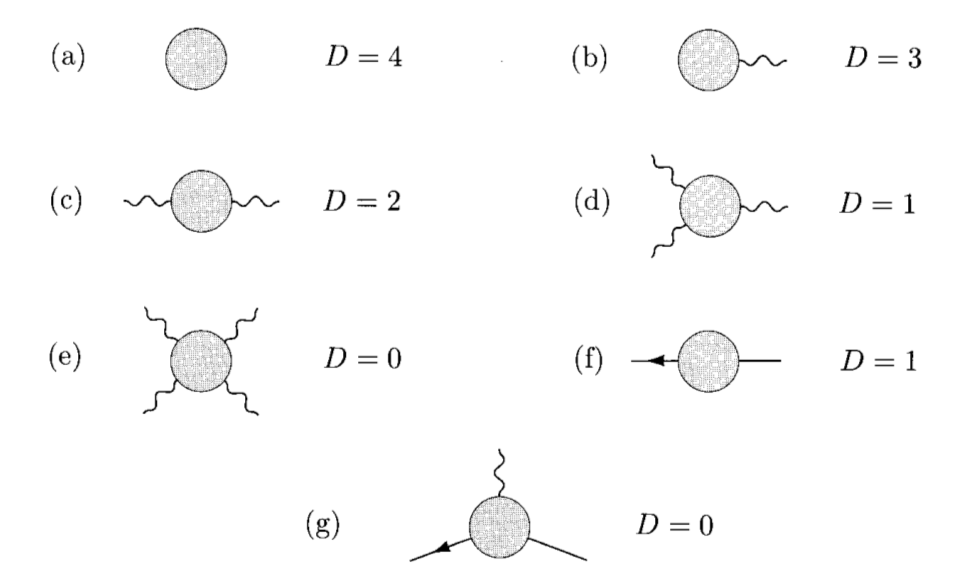
\includegraphics[width=\textwidth]{divergent_diagrams_QED.png}
\caption{The seven QED amplitudes whose superficial degree of divergence (D) is $\geq 0$.}
\label{fig:divergent_diagrams_QED}
\end{figure}


\subsection{How does renormalized perturbation theory relate the bare and physical
masses?}
In renormalized perturbation theory we begin by introducing new fields to rescale the original Lagrangian which only contains bare parameters. The next step is to introduce counterterms containing the physical parameters which splits the Lagrangian into two parts where one part now contains all infinities. The third step is to specify renormalization conditions which then fixes the physical parameters such as mass, charge or field strength. Finally one computes the Feynman amplitudes while maintaining the renormalization condition which yields the counter terms.

The common conditions to specify the physical mass is where the pole of the propagator is, in $\lambda \phi^4$-theory this simply implies that $m^2=p^2$ since the propagator is given by $\dfrac{i}{p^2-m^2+i\epsilon}$. This will define the physical mass $m$ as a function of the bare mass $m_0$ and the mass-counterterm $\delta_m$.

\pagebreak

\section{Renormalization and spontaneous symmetry
breaking}

\subsection{What is spontaneous symmetry breaking? Give a concrete example of a spontaneously broken theory.}
Spontaneous symmetry breaking occurs when the potential term in the Lagrangian has more than one minima which is asymmetric with respect to the Lagrangian. One needs to re-parametrize the Lagrangian around the minima in order to achieve this but this brakes the symmetry of the Lagrangian, i.e. the physical system is asymmetric with respect to an arbitrary minima.

Consider the linear sigma model which is invariant under $\phi^i \rightarrow R^{ij} \phi^j$ implying that it has N symmetries with Lagrangian,

\begin{equation}
L=\dfrac{1}{2}\parentheses{\partial_{\mu}\phi^i}^2 + \mu^2 \parentheses{\phi^i}^2  - \dfrac{\lambda}{4}\left[ \parentheses{\phi^i}^2 \right]^2
\label{eq:linearsigma}
\end{equation}

where the potential term is

\begin{equation}
V \parentheses{\phi^i}=- \mu^2 \parentheses{\phi^i}^2 + \dfrac{\lambda}{4}\left[ \parentheses{\phi^i}^2 \right]^2
\end{equation}

which has it's minimas at $\parentheses{\phi^i_0}^2=\dfrac{\mu^2}{\lambda}$. Re-parametrizing the Lagrangian around one of this minimas breaks the $N$ symmetries and thus the symmetries are spontaneously broken.

\subsection{What is Goldstone's theorem and its implications?}
Goldstone's theorem states that every spontaneously broken symmetry give rise to a massless particles. Thus Goldstone's theorem sets an upper bound for the amount of massive particles in our theory.

In the linear sigma model with $N(N-1)/2$ symmetries, $N-1$ symmetries are broken and the same amount of massless particles are created.

(This implies that spontaneously broken theories can only have one massive particle, e.g. LSW-theory where the only massive particle is the Higgs boson. The $Z$- and $W^\pm$-bosons are massless but are given mass by the Higgs mechanism.)

\subsection{What are the reasons that spontaneously broken theories are renormalizable? (Assuming that the un-broken theory is.)}
Assuming that the unbroken theory is renormalizable the broken theory will also remain renormalizable since the structure of the divergent parts of the Feynman diagrams are unaffected [p.360]. The reparametrization of the Lagrangian will yield several more new divergent diagrams but they all have the same structure and thus all infinities can be absorbed into the same counterterm which renders the broken theory renormalizable as well.

\subsection{What are the basics of Wilson's approach to renormalization?}
The method of Wilson's approach to renormalization follows the following steps:

\begin{itemize}
  \item Introduce high momenta cut-off $\Lambda$
  \item Separate fields into $\hat{\phi}(k)$ where $b\Lambda < |k| < \Lambda$, $0$ otherwise and $\phi(k)$ where $|k|<b\Lambda$, $0$ otherwise and $0<b<1$.
  \item Integrate out  $\hat{\phi}(k)$ to obtain an effective Lagrangian $L_{eff}$
  \item Rescale $L_{eff}$ to obtain recursion relations for all coefficients in the Lagrangian
  \item Iterate through the space of all possible Lagrangians until we find a fixpoint
\end{itemize}
During this procedure some parameters will tend towards zero and thus is not relevant for the theory. 

\subsection{What is the Callan-Symanzik equation and how does it relate to the running of physical quantities?}
Consider a massless theory and introduce the renormalization condition that $p^2=-M^2$ when the dressed (all self-interactions included) propagator is equal to zero. Then the Green's function satisfies the Callan-Symanzik equation
\begin{equation}
\commutator{M \dfrac{\partial}{\partial M} + \beta(\lambda) \dfrac{\partial}{\partial \lambda} + n \gamma(\lambda)}G^{(n)}({x_i};M,\lambda)=0
\label{eq:Callan-Symanzik}
\end{equation} 

It asserts that there exits two universal functions $\beta(\lambda)$ and $\gamma(\lambda)$, related to the shifts in the coupling constants and field strength, that compensates for the shift in the renormalization scale $M$.

The solution of Eq. \eqref{eq:Callan-Symanzik} can be written as

\begin{equation}
G^{(2)}(p,\lambda)= \hat{G}\parentheses{\bar{\lambda}(p;\lambda)} \exp \parentheses{- \int _{p'=M}^{p'=p} d \log (p'/M) 2\commutator{1-\gamma \parentheses{\bar{\lambda}(p;\lambda)}}}
\end{equation}
where $\hat{G}$ is an unknown function through series expansion and $\bar{\lambda}$ is the running coupling constant and it can be shown that it has to satisfy,
\begin{equation}
\frac{d}{d\log(p/M)}\bar{\lambda} (p, \lambda) = \beta (\bar{\lambda}), ~~ \bar{\lambda}(M;\lambda) = \lambda
\label{eq:RG-equations}
\end{equation}
Eq. \eqref{eq:RG-equations} is normally called the renormalization group equation and solving this yields the running constant as function of the momenta and the original coupling constant.

\subsection{Describe how you would chose suitable renormalization conditions.}
We choose renormalization conditions to fix the particle mass at the physical mass as opposed to the bare mass, same for the coupling constant and other bare quantities.

\section{Non-Abelian gauge theory}

\subsection{Why does the requirement of gauge invariance imply the existence of a gauge field?}
It is possible to have a gauge invariant Lagrangian with vector fields, e.g. QED, but when we are interested in creating theories with higher order vector interactions, specifically containing derivatives of vector fields $\partial_{\mu}A^{\mu}$ we run into trouble. The derivative yields extra terms which breaks the gauge invariance. This can be remedied by introducing the covariant derivative

\begin{equation}
D_{\mu}\psi(x)= \partial_{\mu}\psi(x)+ieA_{\mu}\psi(x)
\label{eq:covariantderivative}
\end{equation}
The extra term in Eq. \eqref{eq:covariantderivative} exactly cancels the extra term from the "ordinary" derivative, thus making the replacement $\partial_{\mu} \rightarrow D_{\mu}$ remedies our problem, but at the same time forcing us to introduce a new vector field $A_{\mu}$.

\subsection{What representation do the Yang-Mills gauge field strengths transform according to?}
In the general $SU(N)$ group the covariant derivative transforms as

\begin{equation}
D_{\mu} \rightarrow V D_{\mu} V^{\dagger}
\end{equation}
where $V=\exp \parentheses{i\alpha^{a}(x)t^{a}}$, where $\alpha(x)$ and $f^{abc}$ are structure constants and $t^a$ are the generators of the group. Since $\commutator{D_{\mu}, D_{\nu}}=-igF^{a}_{\mu\nu}t^a$ this implies that 
the Yang-Mills field tensor has the infinitesimal transformation

\begin{equation}
F^{a}_{\mu\nu} \rightarrow F^{a}_{\mu\nu} - f^{abc} \alpha^b F^{c}_{\mu\nu}
\end{equation}
and that the quantity $-\dfrac{1}{4}\parentheses{F^{a}_{\mu\nu}}^2$ appearing in the Yang-Mills Lagrangian is gauge invariant.

\subsection{What are the Yang-Mills equivalents of the Maxwell equations?}
The Yang-Mills equivalents of the Maxwell equations are obtained by applying the Euler-Lagrange equations with respect to $A^{\mu}$ to the Yang-Mills Lagrangian

\begin{equation}
L_{YM}=-\dfrac{1}{4}\parentheses{F^{a}_{\mu\nu}}^2+\bar{\psi} \parentheses{i \slashed{D}-m} \psi
\label{eq:Yang-Mills}
\end{equation}
and are found to be

\begin{equation}
\partial^{\mu} F^{a}_{\mu\nu} + g f^{abc} A^{b\mu} F^{c}_{\mu\nu} = -gj^{a}_{\nu}
\end{equation}
where $j^{a}_{\nu}=\bar{\psi} \gamma_{\nu} t^a \psi$. Eq. \eqref{eq:Yang-Mills} can be rewritten as

\begin{equation}
\parentheses{D^{\mu} F_{\mu\nu}}^a = -g j_{\nu}^{a}
\end{equation}
which in the homogeneous case is called the Bianchi identity

\begin{equation}
\epsilon^{\mu\nu\lambda\sigma} \parentheses{D_{\nu} F_{\lambda\sigma}}^a = 0
\end{equation}
and are non-Abelian equivalence of the homogeneous Maxwell equation.

\subsection{What are the Feynman rules for the Yang-Mills Lagrangian?}
The Feynman rules for the Yang-Mills Lagrangian can be found by expanding the non-Abelian filed tensor in Eq. \eqref{eq:Yang-Mills} and give rise the Feynman rules for the vertices shown in Fig. \ref{fig:Yang-Mills_Feynman_Rules}. The propagators for the fermion and gauge boson respectively are given by

\begin{equation}
\average{\psi_{i\alpha}(x)\bar{\psi}_{j\beta}(y)} = \int \dfrac{d^4k}{(2\pi)^ 4} \parentheses{ \dfrac{i}{\slashed{k} - m}}_{\alpha\beta} \delta_{ij}e^{-ik\cdot (x-y)}
\end{equation}
and 

\begin{equation}
\average{A_{\mu}^{a}(x)A_{\nu}^{b}(y)} = \int \dfrac{d^4k}{(2\pi)^ 4} \parentheses{ \dfrac{-ig_{\mu\nu}}{k^2}} \delta^{ab}e^{-ik\cdot (x-y)}
\end{equation}

\begin{figure}[hbtp]
\centering
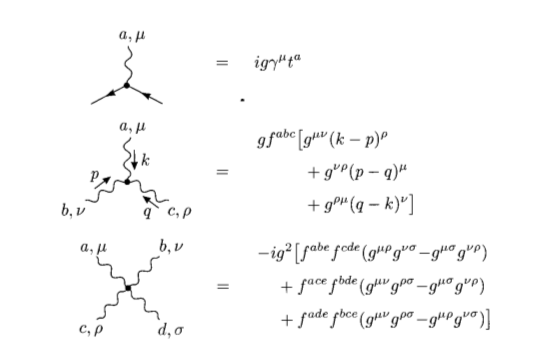
\includegraphics[width=\textwidth]{Non-abelian_Feynman_Rules.png}
\caption{The Feynman rules for the Yang-Mills Lagrangian.}
\label{fig:Yang-Mills_Feynman_Rules}
\end{figure}

\subsection{Why are the coupling constants of the different non-linear terms necessarily equal in Yang-Mills theory?}
There are two ways to approach this question and the first is more hands on: all interaction terms, i.e. non-linear terms, come from the square of the non-Abelian field strength tensor which was a necessity due to non-Abelian gauge invariance. This implies that there is only one coupling constant involved and thus by construction they all have the same coupling constant. 

The other more technical argument is that we expect the Feynman amplitudes to satisfy Ward identities which corresponds to conservation of symmetry currents. This implies that unphysical polarization states are not produced in scattering processes. If one calculates the simple case of fermion-antifermion annihilation into a pair of gauge bosons there is actually Feynman diagrams containing both the fermion-antifermion-boson vertex and the three-boson vertex. Calculations show that the Ward identity can only be satisfied if the coupling constants of the different vertices are equal.

In the same way the diagram for boson-boson scattering includes both the three- and four-boson vertex and the Ward identity can only be satisfied if the coupling constants are equal. These two scattering processes ensures that the coupling constants are equal for the interactions in Fig. \ref{fig:Yang-Mills_Feynman_Rules}.

\subsection{What are Faddeev-Popov ghost fields?}
There is a flaw in the previous argument: we had to assume that a gauge boson was transverse and while this is true in QED this it not necessarily true in a Yang-Mills theory. The Faddeev-Popov procedure 
\begin{equation}
1 = \int D\alpha ~ \delta(G(A^{\alpha}))det\left[ \frac{\delta G}{\delta \alpha}\right]
\end{equation}

give rise to extra terms in the non-Abelian case
\begin{equation}
\frac{\delta G(A^{\alpha})}{\delta \alpha} = \dfrac{1}{g} \partial^{\mu} D_{\mu} 
\end{equation}
which give rise to a ghost Lagrangian

\begin{equation}
L_{ghost}=\bar{c}^a \parentheses{-\partial^2 \delta^{ac} -g \delta^{\mu} f^{abc} A^b_{\mu}}c^c
\end{equation}
These ghost field have the wrong relation between spin and statistics and thus only show up as virtual particles and never as physical observable particles, however they also have the consequence of cancelling the unwanted unphysical polarization states.



\subsection{Questions}
\begin{itemize}
\item Covariant derivative and Christoffel symbols?
\item Differences in Feynman rules for the non-Abelian vertices
\end{itemize}

\section{Running of coupling constant in Yang-Mills theory}

\subsection{How does the introduction of Faddeev-Popov ghosts solve the unitary problem?}

REF: page 516, figure 16.6.

The ghost contribution exactly cancels of the contributions of non-physical gauge bosons. In general the ghost particles serve as negative degrees of freedom to cancel the effects of non-physical polarization states of the gauge bosons.

\subsection{What diagrams contribute to the gauge boson self-energy?}
See Fig. \ref{fig:Gauge_Boson_Self-Energy}.

\begin{figure}[hbtp]
\centering
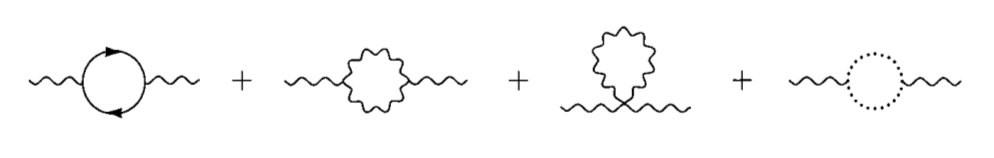
\includegraphics[width=\textwidth]{Gauge_Boson_Self-Energy.png}
\caption{Contributions to the gauge boson self-energy in order $g^2$.}
\label{fig:Gauge_Boson_Self-Energy}
\end{figure}

\subsection{Why is the appearence of gauge fixing parameter $\xi$ not a problem for gauge boson selg-energy? }

The fact that the boson self-energy depends on the gauge does not contradict the general theorem that the S-matrix elements are independent of $\xi$. The reason for this is that the full set of one-loop corrections to a gauge theory S-matrix element always involves a number of different \textit{radiative corrections} to vertices and propagators, the gauge dependence cancels in an intrcate fashion. (at the bottom of page 526) 

\subsection{What is the $\beta$ function of QCD (with the gauge group SU(3))?}

In a general, non-Abelian, gauge theory, the $\beta$ function is given by:

\begin{equation}
\beta(g) = -\frac{g^3}{(4\pi)^2}\left( \frac{11}{3}C_2(G) - \frac{4}{3}n_fC(r) \right)
\end{equation}
where $n_f$ is the number of fermion species in representation $r$, $C(r)$ is the constant from the orthogonality relation:

\begin{equation}
tr[t^a_rt^b_r] = C(r)\delta^{ab}
\end{equation}
which in SU(N) is given by $C(r)= \frac{1}{2}$. Furthermore, $C_2(G)$ is the quadratic Casimir operator of the adjoint representation of the group (group G), which is given by:
\begin{equation}
f^{acd}f^{bcd}=C_2(G)\delta^{ab}
\end{equation}
which in SU(N) is given by $C_2(N)= \frac{N^2-1}{2N}$. Specifically in SU(3) for QCD $\beta$ is given by

\begin{equation}
\beta(g) = -\frac{g^3}{(4\pi)^2} \left( 11 - \frac{2}{3}n_f \right)
\end{equation}
where $n_f$ is now interpreted as the approximately massless quarks.

\subsection{Describe the running coupling constant of SU(3), SU(2) and U(1) respectively.}

By solving the \textit{Renormalization group eq.} (p. 551, $Q=k$): 

\begin{equation}
\frac{d}{d(log(\frac{k}{M}))}\bar{g} = \beta(\bar{g}), \;\;\;\; \bar{g}(M;g) = g,
\end{equation}
we get the solution (p. 541):

\begin{equation}
g^2(k) = \frac{g^2}{1 + \frac{g^2}{(4\pi)^2} \left( \frac{11}{3}N - \frac{2}{3}n_f\right)log(\frac{k^2}{M^2}) }
\end{equation}
for SU(N). This implies that for a sufficiently small $n_f$ (so that that $\beta$ stays negative) non-Abelian gauge theories are asymptotically free (in other world the coupling constant goes to zero as the momenta increases.)


\subsection{How does the renormalization behaviour of QCD depend on the fermion content of the theory?}
The $\beta$-function is, to one-loop order, a sum of the coefficients of the logarithmic divergences of the counter terms which is determined by renormalisation (PoS Eq. (12.54)). In SU(3) for QCD $\beta$ is given by

\begin{equation}
\beta(g) = -\frac{g^3}{(4\pi)^2} \left( 11 - \frac{2}{3}n_f \right)
\end{equation}
which implies that if $n_{f}>16$, QCD is no longer asymptotically free. 


\subsection{Questions}
\begin{itemize}
\item Which are fermion species? Ghost?
\end{itemize}



\section{Quantum Chronodynamics}

\subsection{What are the main issued involved when using perturbation theory in QCD?}

In pertubations theory in QCD the coupling constant is large for small momenta (energy) transfers. Thus our the correction terms do not converge.

\subsection{What are the idea behind the treatment of deep inelastic scattering and why is it a good approximation?}



\subsection{What are the relations that need to be fulfilled by the parton distribution functions?}

The parton distribution function $f_f(\xi)$ is the probability of finding constituent $f$ with longitudinal fraction $\xi$ (part of the total momenta). These have to fulfil:

\begin{equation}
1 = \int_0^1dx~x\left[ f_u(x) + f_d(x) + f_{\bar{u}}(x) + f_{\bar{d}}(x) + f_g(x)\right]
\end{equation}



\subsection{What is a Drell-Yan process and how can it be treated computationally?}

The Drell-Yan procress is when a pair of leptons ($l^+l^-$) with high energy arises from a quark-antiquark annihilation in a proton-proton collision. We relate the cross section computation of this process to the electron pair annihilation to quark-antiquark. For the electro-positron annihilation to hadrons we have:

\begin{equation}
\sigma(e^+e^-\; \rightarrow \; hadrons) = \sigma_0\cdot3\cdot\sum_fQ_f
\end{equation}

The only difference now is between the two calculations is that we mst average rather than sum over tge color orientations of the quark and antiquark. This gives two extra factors of $\frac{1}{3}$

\begin{equation}
\sigma(q_f\bar{q}_f \; \rightarrow \; l^+l^-) = \frac{\sigma_0}{3}Q_f^2
\end{equation}

\subsection{How do mass singularities in QCD scattering processes arise?}

These mass singularities arises from collinear emissions of quarks and/or gluons in QCD. The correction to the order of $\alpha_s$ diverge which in turn give rise to mass singularities. However, in QED these collinear photon emission cancels.

\subsection{How do the parton distribution functions depend on the scale of momentum transfer Q?}

REF eq. 17.128 \\
\\
REF fig 17.21 ?? Kanske ha med?! \\
\\

The Altarelli-Parisi equations predicts the evolution of the parton distribution functions as a functions of the scale of momentum transfer. The parton distribution functions decrease at large $x$ and increase much more rapidly at small $x$ as $Q$ increases. We can picture the proton as having more and more constituents, which share its total momentum.

\end{document}